\begin{flushleft}
	\section{\textcolor{cyan}{Matérial et outillage :}}
	\subsection{\textcolor{green}{Arduino Mega :}}
	L'Arduino Mega est une carte de microcontrôleur basée sur le microcontrôleur ATmega2560. C'est l'une des plus grandes cartes Arduino disponibles, avec 54 broches d'entrée/sortie numériques (dont 15 peuvent être utilisées pour la PWM), 16 entrées analogiques, 4 UART (ports série matériels), un oscillateur à cristal de 16 MHz, une connexion USB, une prise d'alimentation, un en-tête ICSP et un bouton de réinitialisation.
	
	La carte est conçue pour fournir une plateforme plus grande et plus puissante pour des projets plus avancés, et convient particulièrement aux projets nécessitant plus de broches d'entrée/sortie ou plus de puissance de traitement que les autres cartes Arduino peuvent fournir. Elle est compatible avec la plupart des shields Arduino, qui sont des cartes d'extension permettant d'ajouter des fonctionnalités supplémentaires à la carte.
	
	L'Arduino Mega peut être programmé à l'aide du logiciel Arduino, disponible gratuitement sur le site web d'Arduino. Le logiciel comprend un langage de programmation simple basé sur C++ et un ensemble de bibliothèques qui facilitent la communication avec les différentes entrées et sorties de la carte. Avec l'Arduino Mega, vous pouvez créer une large gamme de projets, depuis des clignoteurs LED simples jusqu'à des systèmes robotiques complexes.
	\begin{figure}[h]
		\centering
		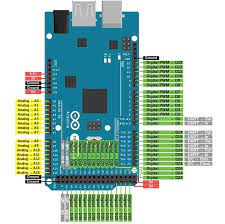
\includegraphics{chapitres/images/ArduinoMega.jpg}
		\caption{Arduino Mega}
		\label{fig:labelname}
	\end{figure}
	\subsection{\textcolor{green}{Bluetooth HC-06 :}}
	Le HC-06 est un module Bluetooth qui permet la communication sans fil entre des appareils électroniques. Il s'agit d'un module couramment utilisé pour la communication sans fil entre des microcontrôleurs et d'autres appareils.
	
	Le HC-06 est un esclave, ce qui signifie qu'il ne peut communiquer qu'avec un appareil maître, tel qu'un smartphone ou un ordinateur, qui initie la communication. Le module fonctionne sur la norme Bluetooth 2.0 et prend en charge une plage de communication allant jusqu'à 10 mètres.
	
	Le HC-06 peut être facilement intégré à un projet, car il ne nécessite que quatre connexions à un microcontrôleur ou à un autre appareil : l'alimentation, la terre, la transmission (TX) et la réception (RX). Une fois connecté, le module peut être configuré à l'aide de commandes AT, qui permettent à l'utilisateur de définir différents paramètres tels que le nom de l'appareil, le débit en bauds et le code d'appariement.
	
	Dans l'ensemble, le HC-06 est une solution polyvalente et économique pour la communication sans fil entre les appareils.
	\begin{figure}[h]
		\centering
		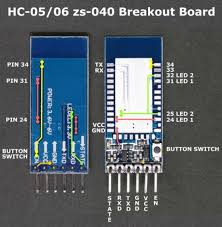
\includegraphics{chapitres/images/bleutouth.jpg}
		\caption{Bluetooth HC-06}
		\label{fig:labelname}
	\end{figure}
	\subsection{\textcolor{green}{ESP8266 :}}
	L'ESP8266 est une micro-puce Wi-Fi à faible coût avec une pile TCP/IP complète et des capacités de microcontrôleur produite par l'entreprise chinoise Espressif Systems. Il a été lancé pour la première fois en 2014 et a rapidement gagné en popularité dans les communautés de fabrication et d'IoT en raison de sa petite taille, de son faible coût et de sa connectivité Wi-Fi intégrée.
	
	L'ESP8266 peut être programmé en utilisant l'IDE Arduino, MicroPython ou d'autres langages de programmation, et est largement utilisé dans une variété de projets IoT tels que l'automatisation domestique, l'éclairage intelligent, les stations météorologiques et la détection à distance. Il dispose d'une gamme de broches GPIO qui peuvent être utilisées pour interfacer avec des capteurs et des actionneurs, et prend en charge une variété de protocoles de communication tels que SPI, I2C et UART.
	
	Il existe plusieurs variantes de l'ESP8266, notamment l'ESP-01, l'ESP-12 et l'ESP-32, chacune avec des broches de connexion, des capacités et des fonctionnalités différentes. L'ESP-32 est une version plus puissante de l'ESP8266, avec des processeurs à double cœur, une connectivité Bluetooth et la prise en charge d'applications plus volumineuses.
	\begin{figure}[h]
		\centering
		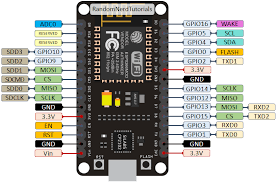
\includegraphics{chapitres/images/esp8266.png}
		\caption{ESP8266}
		\label{fig:labelname}
	\end{figure}
  	\newpage
	\subsection{\textcolor{green}{Raspberry Pi 4 :}}
	Le Raspberry Pi 4 est la quatrième génération d'ordinateur monocarte Raspberry Pi. Il a été lancé en juin 2019 et succède au Raspberry Pi 3B+. Parmi les principales caractéristiques du Raspberry Pi 4, on peut citer :
	
	Broadcom BCM2711 quad-core Cortex-A72 (ARM v8) SoC 64 bits à 1,5 GHz \newline
	2 Go, 4 Go ou 8 Go de SDRAM LPDDR4-3200 (selon le modèle)\newline
	Wi-Fi IEEE 802.11ac 2,4 GHz et 5,0 GHz, Bluetooth 5.0, BLE\newline
	Ethernet Gigabit\newline
	2 ports USB 3.0 ; 2 ports USB 2.0.\newline
	2 ports micro-HDMI (jusqu'à 4kp60 pris en charge)\newline
	Port d'affichage MIPI DSI 2 voies, port de caméra MIPI CSI 2 voies, port audio stéréo à 4 pôles et port vidéo composite\newline
	Graphiques OpenGL ES 3.0\newline
	Décodeur H.265 (4kp60), décodeur H.264 (1080p60), encodeur H.264 (1080p30)\newline
	
	Le Raspberry Pi 4 peut être utilisé pour une large gamme d'applications, notamment en tant qu'ordinateur de bureau, centre multimédia, console de jeu ou pour divers projets DIY. Il fonctionne avec une variété de systèmes d'exploitation, notamment Raspbian, Ubuntu et autres.
	\begin{figure}[h]
		\centering
		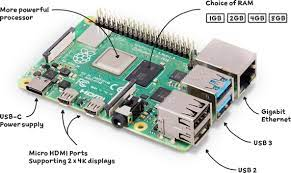
\includegraphics{chapitres/images/raspberry.jpg}
		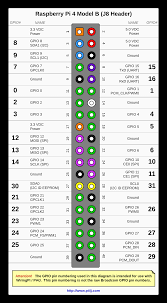
\includegraphics{chapitres/images/raspberryPi.png}
		\caption{Raspberry Pi 4}
		\label{fig:labelname}
	\end{figure}
	\newpage
	\subsection{\textcolor{green}{Mosquitto et Node Red :}}
	Mosquitto et Node-RED sont deux outils de l'écosystème de l'Internet des objets (IoT).
	
	Mosquitto est un broker MQTT (Message Queuing Telemetry Transport) open-source, qui est utilisé pour transférer des données entre des dispositifs IoT. Il peut être utilisé pour collecter et distribuer des données de capteurs, de l'état des dispositifs et d'autres informations pertinentes pour la prise de décision. Mosquitto est souvent utilisé avec Node-RED.
	
	Node-RED est un outil open-source de programmation visuelle pour l'IoT, qui permet de créer des flux de traitement de données pour des dispositifs IoT. Les flux peuvent être créés simplement en faisant glisser et déposer des blocs sur une interface graphique. Node-RED permet de connecter différents dispositifs IoT entre eux, de traiter les données, de les stocker et de les visualiser. Il peut également être utilisé pour envoyer des commandes à des dispositifs, pour automatiser des tâches et pour créer des applications IoT complètes.
	
	En utilisant Mosquitto avec Node-RED, il est possible de collecter des données à partir de dispositifs IoT et de les transférer à Node-RED pour être traitées. Node-RED peut également envoyer des commandes à des dispositifs via Mosquitto. Cette combinaison d'outils est très populaire pour la création de solutions IoT car elle est facile à utiliser et peut être mise en œuvre rapidement.
	\begin{figure}[h]
		\centering
		
\includegraphics{chapitres/images/mosquitto.png}
		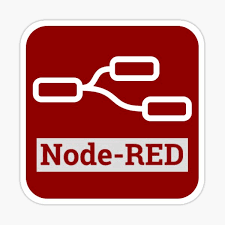
\includegraphics{chapitres/images/nodeRed.png}
		\caption{Mosquitto avec Node-RED}
		\label{fig:labelname}
	\end{figure}
	\newpage
	\subsection{\textcolor{green}{Mit App Inventor :}}
	MIT App Inventor est une plateforme en ligne qui permet aux utilisateurs de créer des applications mobiles pour les appareils Android sans avoir besoin d'apprendre des langages de programmation complexes. Il s'agit d'une interface visuelle de type drag-and-drop qui simplifie le processus de développement d'applications et permet aux utilisateurs de prototyper et de tester rapidement leurs idées. App Inventor utilise un langage de programmation basé sur des blocs, ce qui signifie que les utilisateurs peuvent créer des applications fonctionnelles en connectant visuellement des blocs, plutôt que d'écrire du code traditionnel.
	
	La plateforme a été développée par Google avant d'être transférée au Massachusetts Institute of Technology (MIT) en 2012, où elle a été maintenue et mise à jour par le laboratoire d'informatique et d'intelligence artificielle (CSAIL) du MIT. MIT App Inventor est un logiciel gratuit et open-source, et sa communauté est active dans la création et le partage de ressources pour aider les autres à apprendre et à créer leurs propres applications.
	
	Dans l'ensemble, MIT App Inventor est un excellent outil pour les débutants qui veulent se lancer dans le développement d'applications mobiles sans avoir besoin de connaissances en programmation approfondies.
	\begin{figure}[h]
		\centering
		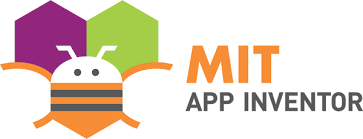
\includegraphics{chapitres/images/AppInventor.png}
		\caption{Mit App Inventor}
		\label{fig:labelname}
	\end{figure}
	\subsection{\textcolor{green}{Conclusion :}}
	Les composants  essentiels pour la construction et la mise en œuvre d'une maison intelligente: 
	
	L'Arduino Mega est une carte microcontrôleur qui peut être programmée pour contrôler les différents capteurs et actionneurs de votre maison intelligente. L'ESP8266 est un module Wi-Fi qui permet de connecter votre système domotique à Internet et de le contrôler à distance. La Raspberry Pi est un ordinateur monocarte qui peut être utilisé pour héberger un serveur Mosquitto, qui est un serveur de messagerie MQTT utilisé pour connecter les différents composants de votre système domotique. Le module Bluetooth HC-06 peut être utilisé pour connecter des appareils Bluetooth tels que des haut-parleurs ou des écouteurs. Les capteurs sont des dispositifs qui peuvent détecter des changements dans l'environnement, tels que la température, l'humidité et la lumière, et envoyer des données à votre système domotique. Node-RED est un outil de programmation graphique qui permet de créer des flux de données pour votre maison intelligente. Enfin, le MIT App Inventor est un environnement de développement d'applications qui permet de créer des applications pour contrôler votre maison intelligente à partir de votre smartphone. En combinant ces composants et outils, vous pouvez créer un système domotique intelligent pour votre maison.
	\newpage
\end{flushleft}
